\begin{filecontents}{shortbib.bib}
@inproceedings{resnet,
  title={Deep residual learning for image recognition},
  author={He, Kaiming and Zhang, Xiangyu and Ren, Shaoqing and Sun, Jian},
  booktitle={Proceedings of the IEEE conference on computer vision and pattern recognition},
  pages={770--778},
  year={2016}
}
\end{filecontents}

\documentclass{article}
\usepackage[margin=1in]{geometry}
\usepackage{hyperref}
\usepackage{amsmath,amsfonts,amssymb,amsthm,commath,dsfont}
\usepackage{enumitem}
\usepackage{framed}
\usepackage{xspace}
\usepackage{microtype}
\usepackage{float}
\usepackage[round]{natbib}
\usepackage{cleveref}
\usepackage[dvipsnames]{xcolor}
\usepackage{graphicx}
\usepackage{listings}
\usepackage[breakable]{tcolorbox}
\tcbset{breakable}
\usepackage{mathtools}
\usepackage{caption}
\usepackage{subcaption}
\usepackage{nicefrac}
\def\b1{\boldsymbol{1}}

\newcommand{\colbar}{\rule[-3mm]{.3mm}{1.5em}}
\newcommand{\rowbar}{\rule[.5ex]{1.5em}{.3mm}}
\DeclareMathOperator{\rank}{rank}
\def\balpha{\boldsymbol{\alpha}}
% following loops stolen from djhsu
\def\ddefloop#1{\ifx\ddefloop#1\else\ddef{#1}\expandafter\ddefloop\fi}
% \bbA, \bbB, ...
\def\ddef#1{\expandafter\def\csname bb#1\endcsname{\ensuremath{\mathbb{#1}}}}
\ddefloop ABCDEFGHIJKLMNOPQRSTUVWXYZ\ddefloop

% \cA, \cB, ...
\def\ddef#1{\expandafter\def\csname c#1\endcsname{\ensuremath{\mathcal{#1}}}}
\ddefloop ABCDEFGHIJKLMNOPQRSTUVWXYZ\ddefloop

% \vA, \vB, ..., \va, \vb, ...
\def\ddef#1{\expandafter\def\csname v#1\endcsname{\ensuremath{\boldsymbol{#1}}}}
\ddefloop ABCDEFGHIJKLMNOPQRSTUVWXYZabcdefghijklmnopqrstuvwxyz\ddefloop

% \valpha, \vbeta, ...,  \vGamma, \vDelta, ...,
\def\ddef#1{\expandafter\def\csname v#1\endcsname{\ensuremath{\boldsymbol{\csname #1\endcsname}}}}
\ddefloop {alpha}{beta}{gamma}{delta}{epsilon}{varepsilon}{zeta}{eta}{theta}{vartheta}{iota}{kappa}{lambda}{mu}{nu}{xi}{pi}{varpi}{rho}{varrho}{sigma}{varsigma}{tau}{upsilon}{phi}{varphi}{chi}{psi}{omega}{Gamma}{Delta}{Theta}{Lambda}{Xi}{Pi}{Sigma}{varSigma}{Upsilon}{Phi}{Psi}{Omega}{ell}\ddefloop

\newcommand\T{{\scriptscriptstyle\mathsf{T}}}
\def\diag{\textup{diag}}

\DeclareMathOperator*{\argmin}{arg\,min}
\DeclareMathOperator*{\argmax}{arg\,max}

\def\SPAN{\textup{span}}
\def\tu{\textup{u}}
\def\R{\mathbb{R}}
\def\E{\mathbb{E}}
\def\Z{\mathbb{Z}}
\def\be{\mathbf{e}}
\def\nf{\nabla f}
\def\veps{\varepsilon}
\def\cl{\textup{cl}}
\def\inte{\textup{int}}
\def\dom{\textup{dom}}
\def\Rad{\textup{Rad}}
\def\lsq{\ell_{\textup{sq}}}
\def\hcR{\widehat{\cR}}
\def\hcRl{\hcR_\ell}
\def\cRl{\cR_\ell}
\def\hcE{\widehat{\cE}}
\def\cEl{\cE_\ell}
\def\hcEl{\hcE_\ell}
\def\eps{\epsilon}
\def\1{\mathds{1}}
\newcommand{\red}[1]{{\color{red} #1}}
\newcommand{\blue}[1]{{\color{blue} #1}}
\def\srelu{\sigma_{\textup{r}}}
\def\vsrelu{\vec{\sigma_{\textup{r}}}}
\def\vol{\textup{vol}}
\def\sr{\sigma_r}
\usepackage{xcolor}

\newcommand{\PA}[1]{\textcolor{red}{PA: #1}}
\newcommand{\ip}[2]{\left\langle #1, #2 \right \rangle}
\newcommand{\mjt}[1]{{\color{blue}\emph\textbf{[M:}~#1~\textbf{]}}}

\newtheorem{fact}{Fact}
\newtheorem{lemma}{Lemma}
\newtheorem{claim}{Claim}
\newtheorem{proposition}{Proposition}
\newtheorem{theorem}{Theorem}
\newtheorem{corollary}{Corollary}
\newtheorem{condition}{Condition}
\theoremstyle{definition}
\newtheorem{definition}{Definition}
\theoremstyle{remark}
\newtheorem{remark}{Remark}
\newtheorem{example}{Example}







\newenvironment{Q}
{%
\clearpage
\item
}
{%
\phantom{s} %lol doesn't work
\bigskip
\textbf{Solution.}
}











\title{CS 446 / ECE 449 --- Homework 3}
\author{\emph{your NetID here}}
\date{Version 1.1}





\begin{document}
\maketitle

\noindent\textbf{Instructions.}
\begin{itemize}
    \item
    Homework is due \textbf{Thursday, March 11, at noon CST}; no late homework accepted.
    
    \item
    Everyone must submit individually on Gradescope under \texttt{hw3} and \texttt{hw3code}.
    
    \item
    The ``written'' submission at \texttt{hw3} \textbf{must be typed}, and submitted in
    any format Gradescope accepts (to be safe, submit a PDF).  You may use \LaTeX, markdown,
    Google Docs, MS word, whatever you like; but it must be typed!
    
    \item
    When submitting at \texttt{hw3}, Gradescope will ask you to mark out boxes
    around each of your answers; please do this precisely!
    
    \item
    Please make sure your NetID is clear and large on the first page of the homework.
    
    \item
    Your solution \textbf{must} be written in your own words.
    Please see the course webpage for full academic integrity information.
    Briefly, you may have high-level discussions with at most 3 classmates,
    whose NetIDs you should place on the first page of your solutions,
    and you should cite any external reference you use; despite all this,
    your solution must be written in your own words.
    
    \item
    We reserve the right to reduce the auto-graded score for
    \texttt{hw3code} if we detect funny business (e.g., your solution
    lacks any algorithm and hard-codes answers you obtained from
    someone else, or simply via trial-and-error with the autograder).
    
    \item The list of library routines with the coding problems are only suggestive.
    
    \item
    When submitting to \texttt{hw3code}, upload \texttt{hw3.py} and \texttt{hw3\_utils.py}.
\end{itemize}

\noindent\textbf{Version History.}
\begin{enumerate}
    \item Initial version.
    \item Corrected typo in Problem 3.
\end{enumerate}

\begin{enumerate}[font={\Large\bfseries},left=0pt]
  


\begin{Q}
    \textbf{\Large ResNet.}

    In this problem, you will implement a simplified ResNet. You do not need to change arguments which are not mentioned here (but you of course could try and see what happens).
    \begin{enumerate}
        \item Implement a class \texttt{Block}, which is a building block of ResNet. It is described in \citep{resnet} Figure 2.

        The input to \texttt{Block} is of shape $(N,C,H,W)$, where $N$ denotes the batch size, $C$ denotes the number of channels, and $H$ and $W$ are the height and width of each channel. For each data example $\vx$ with shape $(C,H,W)$, the output of \texttt{block} is
        \begin{align*}%\label{eq:block}
            \texttt{Block}(\vx)=\sigma_r\del{\vx+f(\vx)},
        \end{align*}
        where $\sigma_r$ denotes the ReLU activation, and $f(\vx)$ also has shape $(C,H,W)$ and thus can be added to $\vx$. In detail, $f$ contains the following layers.
        \begin{enumerate}
            \item A \texttt{Conv2d} with $C$ input channels, $C$ output channels, kernel size 3, stride 1, padding 1, and no bias term.
            \item A \texttt{BatchNorm2d} with $C$ features.
            \item A ReLU layer.
            \item Another \texttt{Conv2d} with the same arguments as i above.
            \item Another \texttt{BatchNorm2d} with $C$ features.
        \end{enumerate}
        Because $3\times3$ kernels and padding 1 are used, the convolutional layers do not change the shape of each channel. Moreover, the number of channels are also kept unchanged. Therefore $f(\vx)$ does have the same shape as $\vx$.

        Additional instructions are given in doscstrings in \texttt{hw3.py}.
        
        \textbf{Suggested Library routines:} \texttt{torch.nn.Conv2d and torch.nn.BatchNorm2d.}

        \item Explain why a \texttt{Conv2d} layer does not need a bias term if it is followed by a \texttt{BatchNorm2d} layer.

        \item Implement a (shallow) \texttt{ResNet} consists of the following parts:
        \begin{enumerate}
            \item A \texttt{Conv2d} with 1 input channel, $C$ output channels, kernel size 3, stride 2, padding 1, and no bias term.
            \item A \texttt{BatchNorm2d} with $C$ features.
            \item A ReLU layer.
            \item A \texttt{MaxPool2d} with kernel size 2.
            \item A \texttt{Block} with $C$ channels.
            \item An \texttt{AdaptiveAvgPool2d} which for each channel takes the average of all elements.
            \item A \texttt{Linear} with $C$ inputs and 10 outputs.
        \end{enumerate}
        Additional instructions are given in doscstrings in \texttt{hw3.py}.
        
        \textbf{Suggested Library routines:} \texttt{torch.nn.Conv2d, torch.nn.BatchNorm2d, torch.nn.MaxPool2D, }
        \texttt{torch.nn.AdaptiveAvgPool2d and torch.nn.Linear.}
        
        
        
        \textbf{Remark:} The \texttt{epoch\_loss} and \texttt{fit\_and\_evaluate} routines of \texttt{hw2} can be used to train your ResNet model. It is not required for you to do so for the purpose of this problem.
    \end{enumerate}
\end{Q}

   
          \begin{Q}
             \textbf{\Large Decision Trees.}

              Consider the training and testing data sets as given in Figures~\ref{fig: training 1} and~\ref{fig: testing 1} for the sub-parts (a)-(c). For the sub-parts (d) \& (e), refer to the training and testing data sets as given in Figures~\ref{fig: training 2} and~\ref{fig: testing 2}.
              \begin{figure}[h]
                \centering
                \begin{subfigure}{0.49\columnwidth}
                \centering
                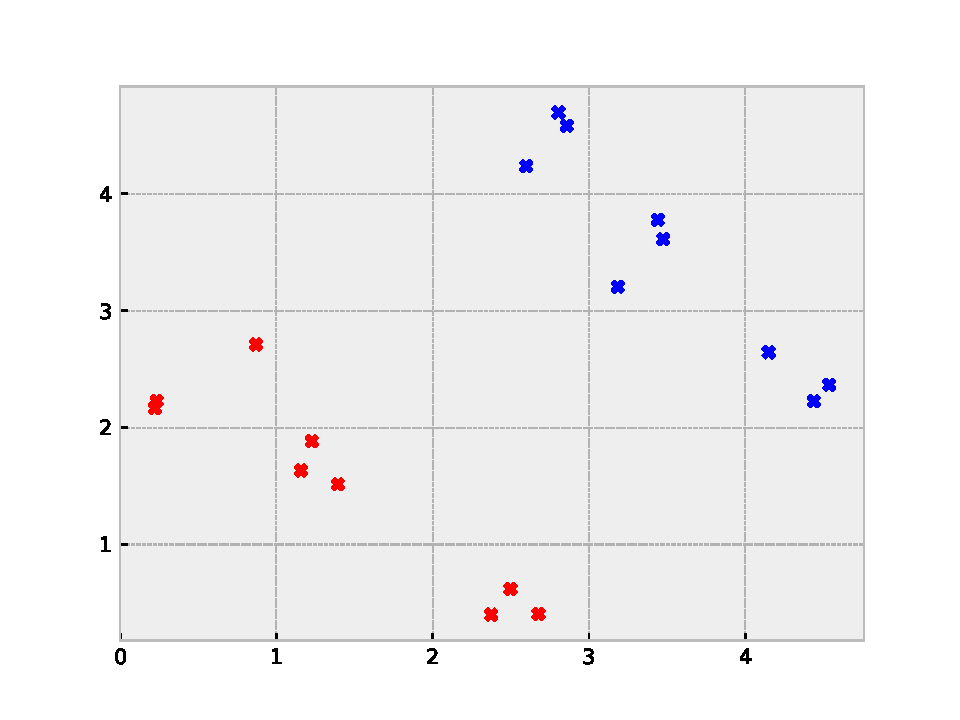
\includegraphics[width=0.99\columnwidth]{figures/training.pdf}
                \caption{Fig 1a: Training data set 1.}
                \label{fig: training 1}
                \end{subfigure}
                \begin{subfigure}{0.49\columnwidth}
                \centering
                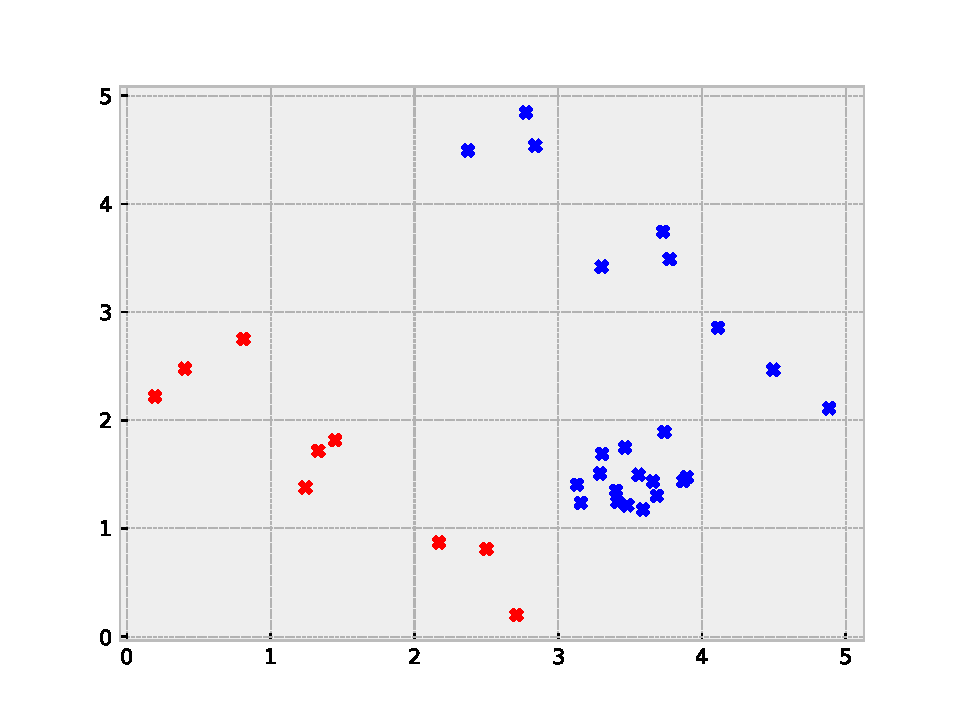
\includegraphics[width=0.99\columnwidth]{figures/testing.pdf}
                \caption{Fig 1b: Testing data set 1.}
                \label{fig: testing 1}
                \end{subfigure}
                \end{figure}
            \begin{enumerate}
              \item Describe a decision tree of depth one with integral
                and axis-aligned decision boundaries
                which achieves error at most $\frac 1 6$ on training data set 1 (\Cref{fig: training 1}).
              \item Describe a decision tree (of any depth) with integral
                and axis-aligned decision boundaries
                which achieves zero error on training data set 1 (\Cref{fig: training 1}).

              \item Describe a decision tree (of any depth) with integral
                and axis-aligned decision boundaries
                which achieves zero error on training data set 1 (\Cref{fig: training 1})
                but has error at least $\frac 1 4$ on 
                testing data set 1 (\Cref{fig: testing 1}).

                \clearpage
            
             \item
              \begin{figure}[h]
                \centering
                \begin{subfigure}{0.49\columnwidth}
                \centering
                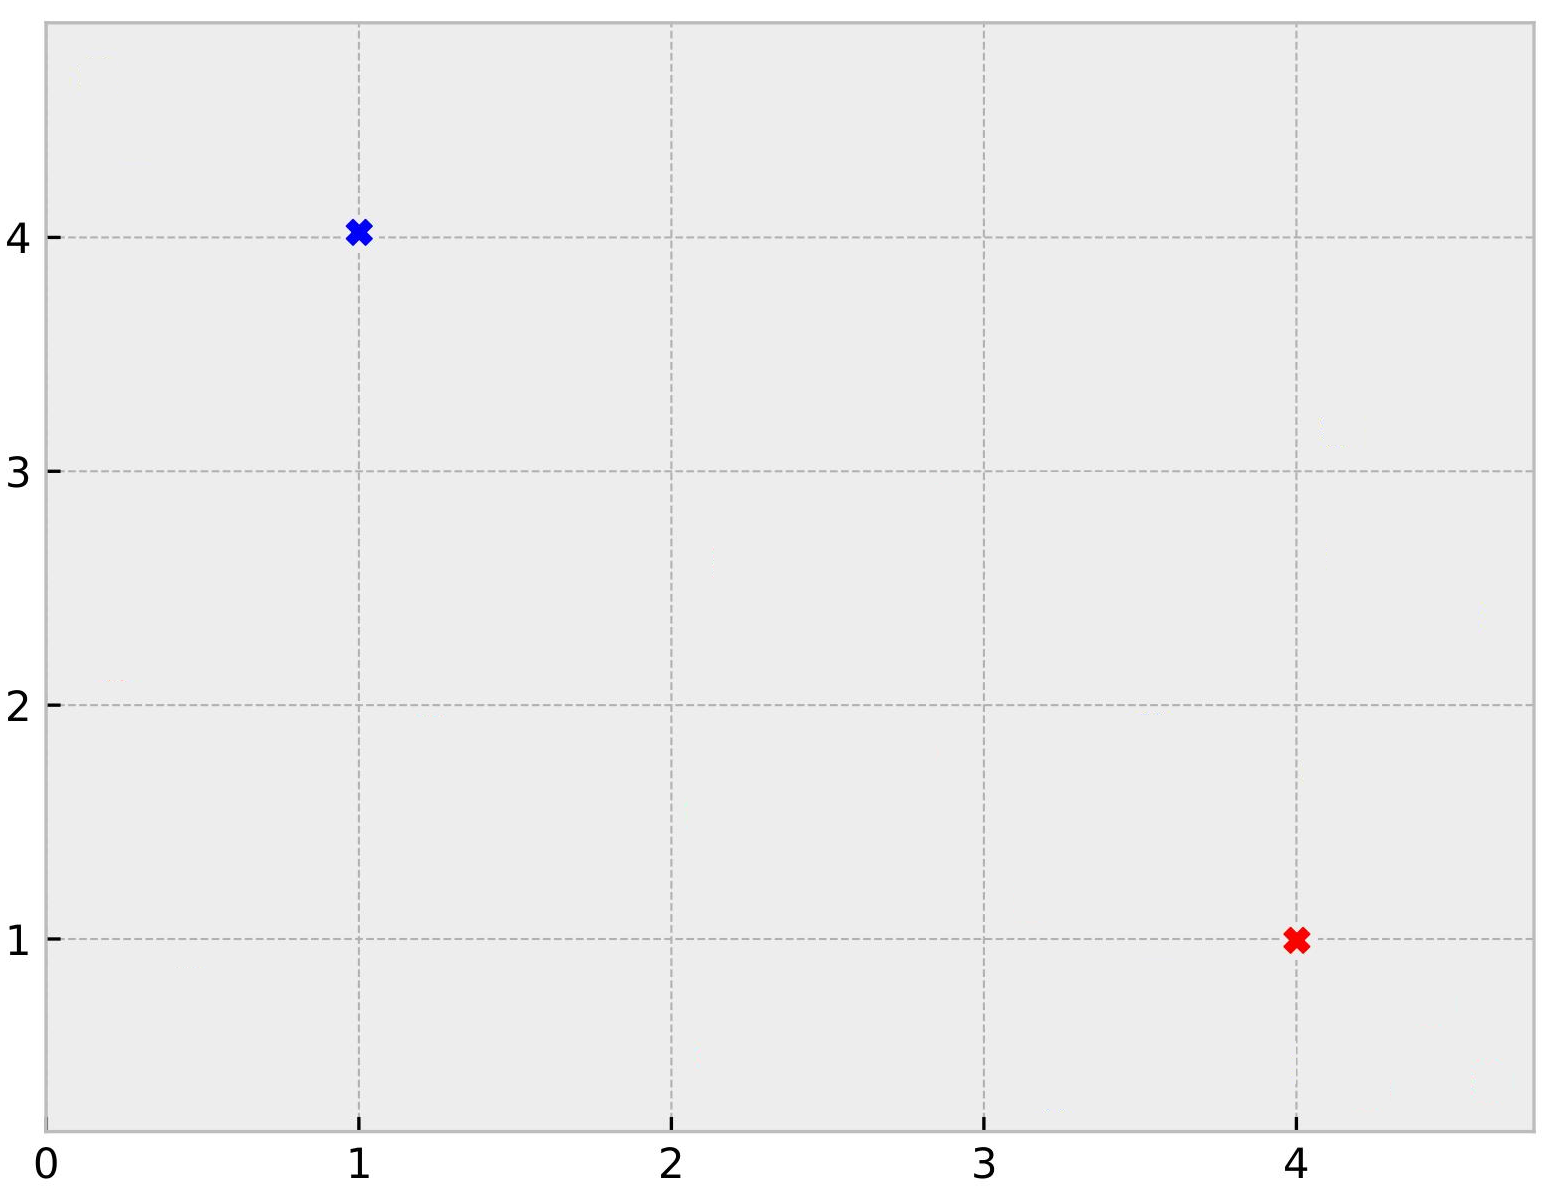
\includegraphics[width=0.85\columnwidth]{figures/training_new.png}
                \caption{Fig 2a: Training data set 2.}
                \label{fig: training 2}
                \end{subfigure}
                \begin{subfigure}{0.49\columnwidth}
                \centering
                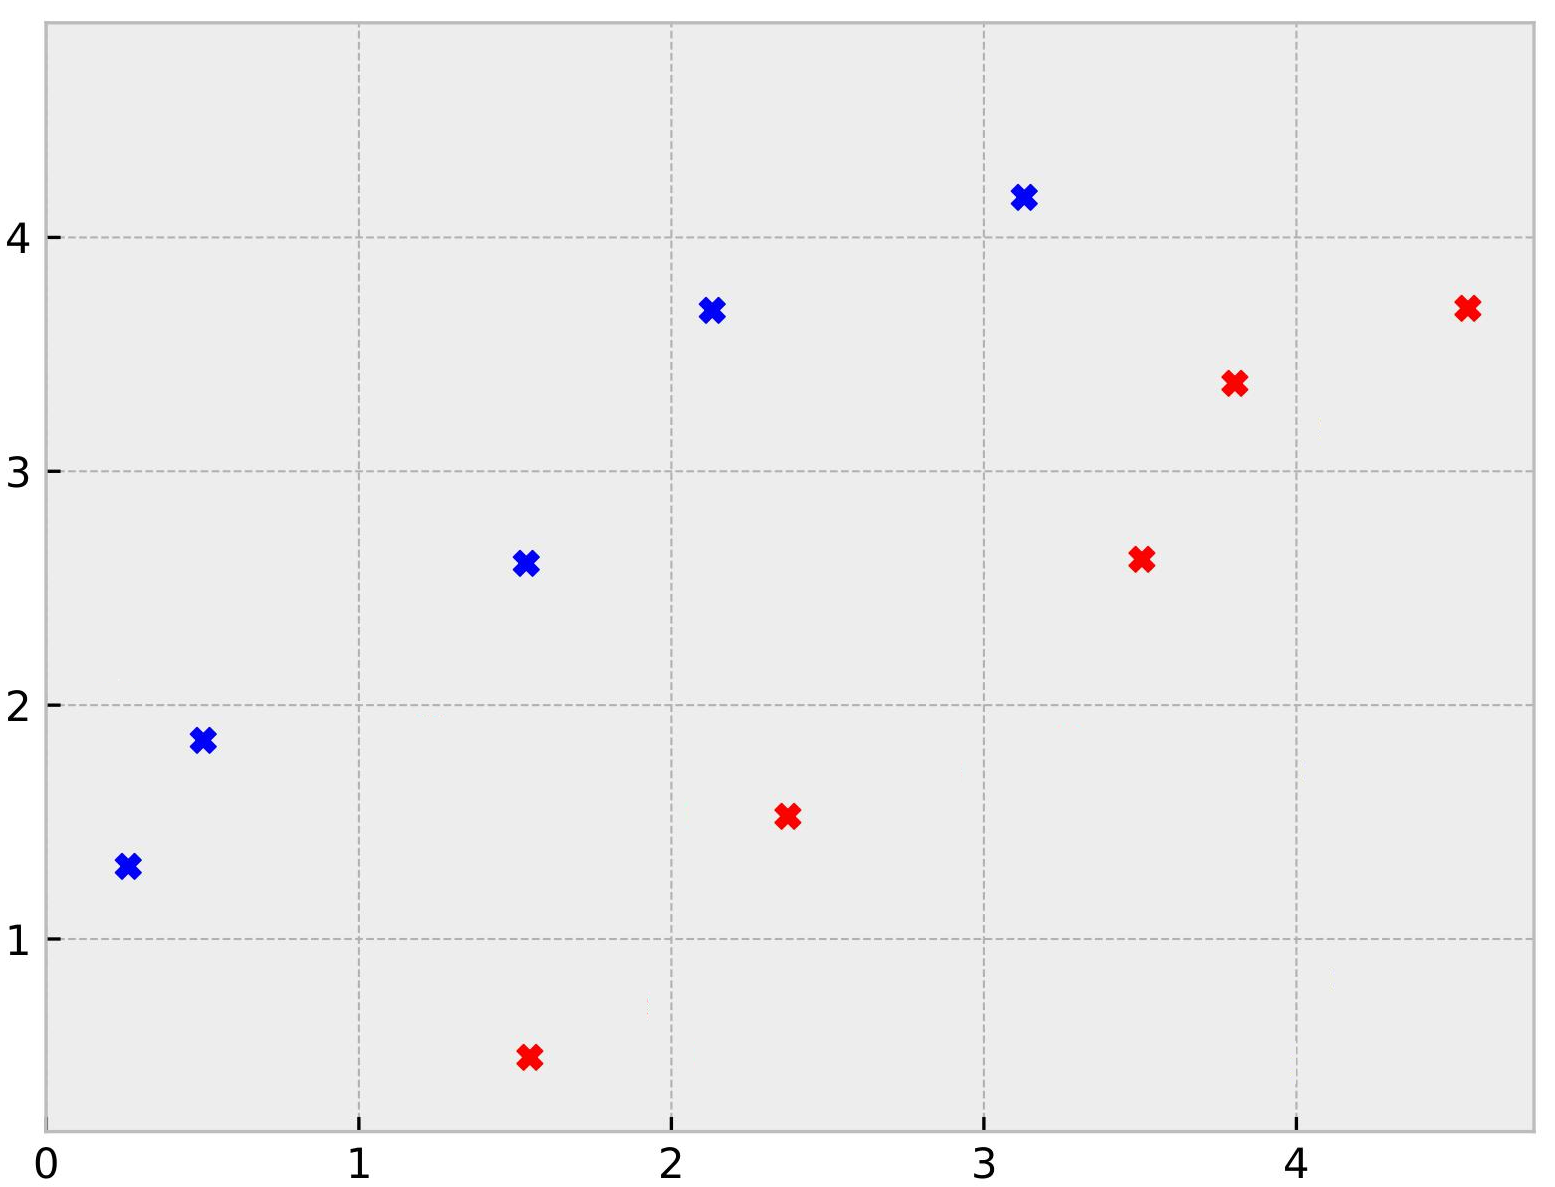
\includegraphics[width=0.85\columnwidth]{figures/test_new.png}
                \caption{Fig 2b: Testing data set 2.}
                \label{fig: testing 2}
                \end{subfigure}
              \end{figure}

              Describe a decision tree with integral and axis-aligned decision boundaries with at most two splits, which achieves zero error on training data set 2 and calculate its error on testing data set 2.
              
              \item Construct a 1-nn classifier using training data set 2 and state its error on testing data set 2.
              
              
              \textbf{Remark:} Note that \emph{every} decision tree (axis aligned integral splits) with at most two splits has positive test error in this problem. Therefore one nearest neighbor is a better choice here.
          
            
            
            
            \end{enumerate}
          \end{Q}



          \begin{Q}
    	  \textbf{\Large Nearest Neighbor.}

          \begin{enumerate}
          \item Implement the 1-nearest neighbor algorithm in the \texttt{one\_nearest\_neighbor()} function in \texttt{hw3.py}. In the starter code you are given three torch tensors as input:
    	\begin{itemize}
    	  \item \texttt{X} - training set
    	  \item \texttt{Y} - training labels
          \item \texttt{X\_test} - testing set
          \end{itemize}
          Use the training set to determine labels for the testing set. Return the labels for the testing set as determined by your nearest neighbor implementation.
          \item Plot the Voronoi diagram of your nearest neighbor results. Use the data set returned from \texttt{load\_one\_nearest\_neighbor\_data()} in \texttt{hw3\_utils.py}. You may use the function \texttt{voronoi\_plot()} provided to you in \texttt{hw3\_utils.py} to help generate the diagram.  There is no need to submit code for this part, only submit the plots in the written portion.
          \end{enumerate}
          \end{Q}
\begin{Q}
   \textbf{\Large Robustness of the Majority Vote Classifier.}\\
   \def\maj{\textsc{Maj}}

    
    The purpose of this problem is to further investigate the behavior of the majority vote classifier (\textit{Slide 5, Lecture 12}) using Hoeffding's inequality (\textit{Slide 20, Lecture 13; will be included in Lecture 12}).  Simplified versions of Hoeffding's inequality are as follows.
     \begin{theorem}\label{thm: hoeffding}
       Given independent random variables $(Z_1,\ldots,Z_k)$ with $Z_i \in [0,1]$,
         \begin{equation}\label{eq: hoeffding 1}
           \Pr\sbr{\sum_{i=1}^k Z_i \geq  \sum_{i=1}^k\mathbb{E}[Z_i] + k\eps } \leq \exp\del{-2k\eps^2},
         \end{equation}
         and
         \begin{equation}\label{eq: hoeffding 2}
           \Pr\sbr{\sum_{i=1}^k Z_i \leq  \sum_{i=1}^k\mathbb{E}[Z_i] - k\eps } \leq \exp\del{-2k\eps^2}.
         \end{equation}
     \end{theorem}

     In this problem we have an odd number $n$ of classifiers $(f_1,\ldots,f_n)$
     and only consider their behavior
     on a fixed data example $(x,y)$; by classifier we mean $f_i(x) \in \{\pm 1\}$.
     Define the majority vote classifer $\maj$ as
     \[
       \maj(x)
       := 2\cdot \1\sbr{\sum_{i=1}^n f_i(x) \geq 0 } - 1
       = \begin{cases}
           +1 &\sum_{i=1}^n f_i(x) > 0, \\
           -1 &\sum_{i=1}^n f_i(x) < 0,
         \end{cases}
     \]
     where we will not need to worry about ties since $n$ is odd.

     To demonstrate the utility of \Cref{thm: hoeffding} in analyzing $\maj$, suppose
     that $\Pr[ f_i(x) = y ] = p > 1/2$ independently for each $i$.
     Then, by defining a random variable $Z_i := \1[ f_i(x) \neq y]$
     and noting $\bbE Z_i = 1 - p$,
     \begin{align*}
       \Pr[\maj(x) \neq y]
       &=
       \Pr\sbr{ \sum_{i=1}^n \1[ f_i(x) \neq y] \geq \frac n 2 }
       \\
       &=
       \Pr\sbr{ \sum_{i=1}^n Z_i \geq n(1-p) - \frac n 2 + np }
       \\
       &=
       \Pr\sbr{ \sum_{i=1}^n Z_i \geq n \bbE Z_1 + n(p-1/2) }
       \\
       &\leq
       \exp\del{ -2n(p-1/2)^2 }.
     \end{align*}
     The purpose of this problem is to study the behavior of $\maj(x)$ when not all of the classifiers $(f_1,\ldots,f_n)$ are independent.
     \begin{enumerate}
       \item
         Assume $n$ is divisible by $6$ and $5n/6$ is odd,
         and that of the $n$ classifiers $(f_1,\ldots,f_n)$,
         now only $5n/6$ of them have independent errors on $x$,
         specifically $\Pr[f_i(x) = y] = p := 4/5$ for $5n/6$ of the classifiers.
         By contrast, make no assumption on the other $n/6$ classifiers and their errors. Now use Hoeffding's inequality to show that the majority vote classifier
         over all $n$ classifiers is still good, specifically showing
         \[
           \Pr\sbr{ \maj(x) \neq y } \leq \exp(-n / 15).
         \]

    \textbf{Remark:} This problem shows that even with corruption levels more than 16\%, the robustness of the majority vote classifier allows for a reasonable probability of correctness for sufficiently large $n$.
  
  \textbf{Hint:} Use Hoeffding's inequality (Eq~(\ref{eq: hoeffding 1})) on the $5n/6$ classifiers which have independent errors. However, in this case the majority vote can be incorrect when less than half of the $\frac{5n}{6}$ (independent) classifiers are in error, due to the arbitrary behavior of the remaining $\frac{n}{6}$ classifiers. A good point to start is by modifying the calculations for $\Pr[\maj(x) \neq y]$ in the preamble of this problem.
  
  \textbf{For full points:} You need to derive the inequality $\Pr\sbr{ \maj(x) \neq y } \leq \exp(-n / 15)$ rigorously for ANY possible behavior of the $\frac{n}{6}$ arbitrary classifiers.


       \item
         Suppose again that $n$ is divisible by $5$ and $3n/5$ is odd,
         but now that only $3n/5$ of the classifiers have independent errors,
         and are correct with probability $\Pr[f_i(x) = y] = p:=2/3$.  Describe malicious behavior for the remaining $2n/5$ classifiers so that
         \[
           \Pr\sbr{ \maj(x) = y } \leq \exp(-n / 30).
         \]

\textbf{Remark:} This problem shows that the performance of the majority vote classifier degrades significantly with higher corruption levels and increased probability of error.
  
  \textbf{Hint:} This may require the use of ``reverse'' form of Hoeffding's inequality, i.e., Eq~(\ref{eq: hoeffding 2}) of Theorem~\ref{thm: hoeffding}. First, specify the malicious behavior of the $\frac{2n}{5}$ arbitrary classifiers. Consider various deterministic choices for the malicious behavior as potential candidates.
  
  \textbf{For full points:} Describe the malicious behavior of the arbitrary classifiers AND derive the inequality $\Pr\sbr{ \maj(x) = y } \leq \exp(-n / 30)$.
         
     \end{enumerate}

\end{Q}
  


\end{enumerate}
\clearpage
\bibliography{shortbib}
\bibliographystyle{plainnat}

\end{document}
